\documentclass[10pt,a4paper]{article}
\usepackage[utf8]{inputenc}
\usepackage[T1]{fontenc}
\usepackage{lmodern}
\usepackage[margin=1.5cm, top=1.4cm, bottom=1.4cm]{geometry}
\usepackage{hyperref}
\usepackage{enumitem}
\usepackage{titlesec}
\usepackage{xcolor}
\usepackage{graphicx}

\definecolor{accent}{HTML}{00686E}
\hypersetup{colorlinks=true, urlcolor=accent, linkcolor=accent}
\pagenumbering{arabic}
\setlength{\parindent}{0pt}

\titleformat{\section}{\large\bfseries\color{accent}}{}{0em}{}[\vspace{-0.6em}\rule{\textwidth}{0.8pt}]
\titlespacing{\section}{0pt}{7pt}{4pt}

\newcommand{\role}[4]{%
  \textbf{#1} \hfill \textbf{#2}\\[1pt]%
  \textit{#3} \hfill \textit{#4}\\[2pt]%
}
\setlist[itemize]{leftmargin=1.2em, itemsep=1.5pt, topsep=2pt, parsep=0pt}

\begin{document}

% ================= HEADER =================
\begin{minipage}[c]{0.80\textwidth}
  {\Huge\bfseries Prabhavit Gupta}\\[3pt]
  {\color{accent}\large Agentic AI Developer: Autonomous Agents, LangGraph \& MCP}\\[6pt]
  {\footnotesize +39 351 610 7807 ~$\vert$~
  \href{mailto:prabhavitg@gmail.com}{prabhavitg@gmail.com} ~$\vert$~
  \href{https://www.linkedin.com/in/prabhavit/}{linkedin.com/in/prabhavit} ~$\vert$~
  \href{https://github.com/prab-gupta}{github.com/prab-gupta} ~$\vert$~
  Venice, Italy (CET Time Zone / EU Permanent Resident / Available Immediately)}
\end{minipage}\hfill
\begin{minipage}[c]{0.18\textwidth}
  \raggedleft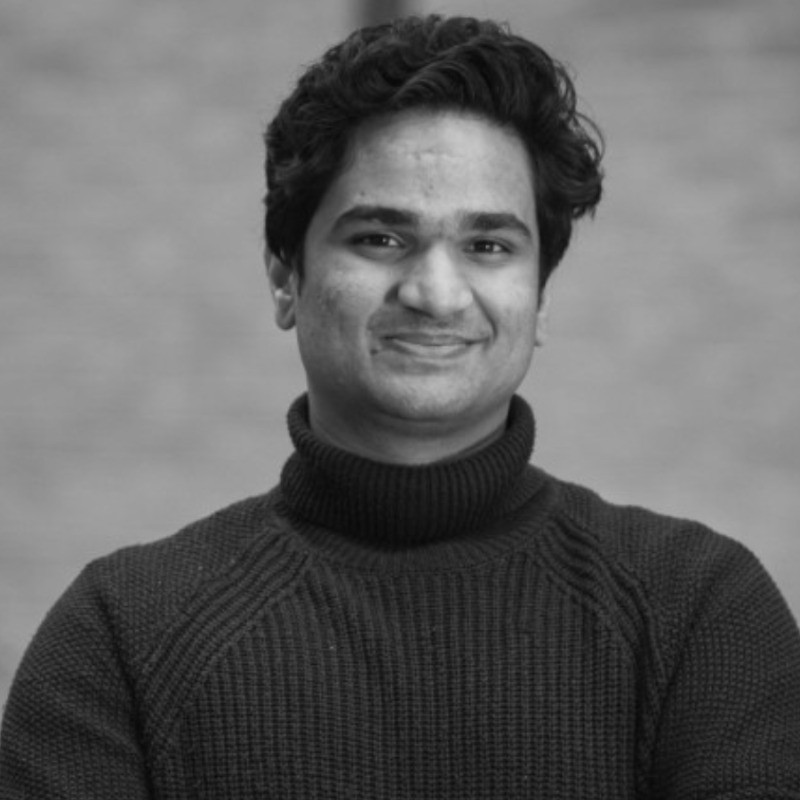
\includegraphics[width=2.0cm]{photo.jpg}
\end{minipage}
\vspace{-2pt}

% ================= SUMMARY =================
\section{Summary}
Agentic AI Systems Engineer with 3 years of commercial production experience architecting autonomous multi-agent loops, state graph workflows, and enterprise tool-calling integrations. Deep hands-on expertise building production systems using LangGraph, LangChain, and Model Context Protocol (MCP), enabling LLMs (Claude 3.5 Sonnet, GPT-4o) to reason, plan, invoke external APIs, and execute complex workflows independently. Proven track record implementing short- and long-term memory structures, schema validation guardrails, and automated evaluation harnesses that eliminate hallucinations and rogue execution paths. Dedicated and proactive engineer available immediately for full-time remote roles without notice period.

% ================= TECHNICAL EXPERTISE =================
\section{Technical Expertise}
\begin{itemize}
  \item \textbf{Agentic Frameworks \& Runtimes:} LangGraph (state machines, cyclical loops), LangChain, AutoGen, CrewAI, Model Context Protocol (MCP), Anthropic Tool Use, OpenAI Function Calling.
  \item \textbf{Reasoning \& Memory Management:} Chain-of-thought reasoning, self-reflection, planning agents, long-term vector memory (Qdrant, Pinecone, Chroma), conversational state persistence with Redis.
  \item \textbf{Tool \& API Integrations:} Exposing enterprise RESTful APIs and databases to agents, strict Pydantic payload validation, sandboxed execution, rate-limiting, and error recovery.
  \item \textbf{Safety Guardrails \& Evaluation:} NeMo Guardrails, automated evaluation suites (prompt regression, tool misuse detection, cost/token tracking), human-in-the-loop approvals.
  \item \textbf{Backend \& Infrastructure:} Python (asyncio, FastAPI, httpx), Docker containerization, PostgreSQL, Redis, Linux headless server administration.
  \item \textbf{Languages \& Availability:} English (C1 Professional, fluent), Hindi (Native), Italian (Conversational). Available immediately without notice period.
\end{itemize}

% ================= EXPERIENCE =================
\section{Experience}

\role{\href{https://flowspace.co}{FlowSpace.co}}{Mar 2024 - Aug 2026}{Lead Agentic AI Engineer \& Forward Deployed Architect}{London, UK (remote)}
\begin{itemize}
  \item Designed and deployed autonomous multi-agent orchestration systems in Python using LangGraph and MCP, automating complex multi-step data workflows for 4,500+ enterprise users.
  \item Built custom Model Context Protocol (MCP) servers exposing internal databases and 15+ external cloud services to Claude 3.5 Sonnet and GPT-4o with strict schema enforcement.
  \item Implemented stateful short-term and long-term memory architectures using Redis and vector search, enabling agents to maintain context across multi-turn sessions.
  \item Established automated evaluation pipelines and guardrails monitoring tool invocation accuracy, reducing unauthorized actions and hallucinations to under 0.2\%.
  \item Optimized asynchronous execution loops and semantic caching, decreasing median agent response latency by 35\% and lowering token consumption.
\end{itemize}

\role{Urlink}{Apr 2025 - Jul 2025}{AI Systems \& Platform Developer (Freelance)}{Barcelona, Spain (remote)}
\begin{itemize}
  \item Developed automated LLM agent workflows in Python that dynamically query external REST APIs, validate responses via Pydantic, and write normalized records to databases.
  \item Implemented error handling, exponential backoff retries, and token rate-limiting across multi-tenant agent execution threads.
  \item Created comprehensive test suites with pytest and Playwright to verify deterministic behavior and schema adherence across agent tool invocations.
\end{itemize}

\role{Independent Technical Consultant}{Aug 2023 - Feb 2024}{Applied AI Developer}{Venice, Italy}
\begin{itemize}
  \item Built autonomous task automation prototypes and document analysis agents for European SMB clients using LangChain and OpenAI APIs.
  \item Deployed containerized agent microservices on remote Linux VPS instances using Docker and systemd daemons.
  \item Authored technical architecture runbooks and integration specifications for client engineering leadership.
\end{itemize}

% ================= EDUCATION =================
\section{Education}
\role{Ca' Foscari University of Venice}{2020 - 2024}{BA in Philosophy, International Studies and Economics}{Venice, Italy}
\begin{itemize}
  \item Rigorous training in formal logic, statistical inference, quantitative economics, and complex systems modeling.
\end{itemize}

\end{document}
